\section{Лекция 14}

\subsection{Монотонность и экстремумы функций}

\begin{theorem} 
    $f: \useg{a, b} \to \R, f $ -- непрерывна на $\useg{a, b}$, $f$ диффиренцируема на $(a, b)$

    \begin{enumerate}
        \item $f$ возрастает на $\useg{a, b} \Longleftrightarrow f' \geqslant 0 $ на $(a, b)$ 
        \item $f$ убывает на $\left\langle {a,b} \right\rangle \Longleftrightarrow f'  \leqslant 0 $ на $(a, b)$ 
        \item $f$ постоянна на $\left\langle {a,b} \right\rangle  \Longleftrightarrow f' = 0 $ на $(a, b)$ 
    \end{enumerate}

\end{theorem}

\begin{proof} \quad
    \begin{enumerate}
        \item $\ola$ $f \inc \Longleftrightarrow \forall x, y \in \useg{a, b} \,\, \frac{f(x) - f(y)}{x - y} \geqslant 0 \Rightarrow f' \geqslant 0$. \\\\
        $\ora$ $f' \geqslant 0 \Rightarrow \frac{f(x)-f(y)}{x-y} = f'(\theta), \theta \in (a, b)$ (по теореме Лагранжа).
        \item[2--3.] Аналогично
    \end{enumerate}
\end{proof}

\begin{remark}
    Как описать строгое возрастание? 
\end{remark}

$\ok$ $f' > 0$ на $(a, b) \Rightarrow f $ строго возрастает на $\useg{a, b} $
\\\\
$\but$ $f' > 0$ на $(a, b) \not\Leftarrow f $ строго возрастает на $\useg{a, b} ($контрпример $f(x) = x ^ 3)$ 

\begin{flalign*}
    f \text{\,строго возрастает} 
    \Longleftrightarrow
    \begin{cases}
        \forall I \subset (a, b) \; \exists \; x \in I : f'(x) > 0 \\
        f'(x) \geqslant 0
    \end{cases} && 
\end{flalign*}  

\quad 

\quad 

\quad
\subsection{Выпуклые функции}

\begin{definition}
    $f : \useg{a, b} \to \R $ -- выпуклая на $\useg{a,b}$, если $\forall x_1, x_2 \in \useg{a,b}, \forall \lambda \in (0, 1) \Rightarrow  \\f(\lambda x_1 + (1 - \lambda) x _ 2) \leqslant \lambda f(x_1) + (1 - \lambda) f (x _ 2)$
\end{definition}




\quad
\tikzset{every picture/.style={line width=0.75pt}} %set default line width to 0.75pt        

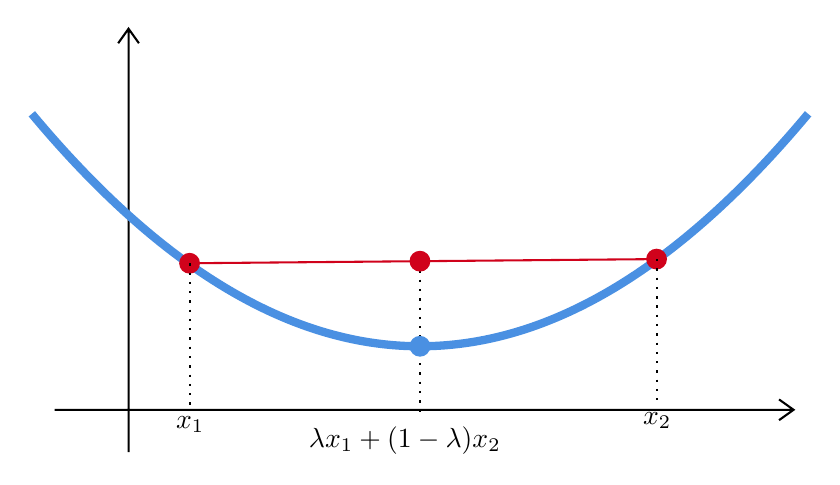
\begin{tikzpicture}[x=0.75pt,y=0.75pt,yscale=-1,xscale=1]
%uncomment if require: \path (0,300); %set diagram left start at 0, and has height of 300

%Shape: Axis 2D [id:dp13272711467424314] 
\draw  (50,248.6) -- (406,248.6)(85.6,65) -- (85.6,269) (399,243.6) -- (406,248.6) -- (399,253.6) (80.6,72) -- (85.6,65) -- (90.6,72)  ;
%Shape: Parabola [id:dp976320101259972] 
\draw  [color={rgb, 255:red, 74; green, 144; blue, 226 }  ,draw opacity=1 ][line width=3]  (39,106) .. controls (163.67,255.33) and (288.33,255.33) .. (413,106) ;
%Straight Lines [id:da25515767039946025] 
\draw [color={rgb, 255:red, 208; green, 2; blue, 27 }  ,draw opacity=1 ]   (115,178) -- (340,176) ;
%Shape: Circle [id:dp5228763574022932] 
\draw  [color={rgb, 255:red, 208; green, 2; blue, 27 }  ,draw opacity=1 ][fill={rgb, 255:red, 208; green, 2; blue, 27 }  ,fill opacity=1 ] (110.5,178) .. controls (110.5,175.51) and (112.51,173.5) .. (115,173.5) .. controls (117.49,173.5) and (119.5,175.51) .. (119.5,178) .. controls (119.5,180.49) and (117.49,182.5) .. (115,182.5) .. controls (112.51,182.5) and (110.5,180.49) .. (110.5,178) -- cycle ;
%Shape: Circle [id:dp6463819878430874] 
\draw  [color={rgb, 255:red, 208; green, 2; blue, 27 }  ,draw opacity=1 ][fill={rgb, 255:red, 208; green, 2; blue, 27 }  ,fill opacity=1 ] (335.5,176) .. controls (335.5,173.51) and (337.51,171.5) .. (340,171.5) .. controls (342.49,171.5) and (344.5,173.51) .. (344.5,176) .. controls (344.5,178.49) and (342.49,180.5) .. (340,180.5) .. controls (337.51,180.5) and (335.5,178.49) .. (335.5,176) -- cycle ;
%Straight Lines [id:da0562686555250248] 
\draw  [dash pattern={on 0.84pt off 2.51pt}]  (115,178) -- (115,249) ;
%Straight Lines [id:da3535183278825579] 
\draw  [dash pattern={on 0.84pt off 2.51pt}]  (340,176) -- (340,247) ;
%Straight Lines [id:da20443057247970886] 
\draw  [dash pattern={on 0.84pt off 2.51pt}]  (226,177) -- (226,251) ;
%Shape: Circle [id:dp9860332203810883] 
\draw  [color={rgb, 255:red, 208; green, 2; blue, 27 }  ,draw opacity=1 ][fill={rgb, 255:red, 208; green, 2; blue, 27 }  ,fill opacity=1 ] (221.5,177) .. controls (221.5,174.51) and (223.51,172.5) .. (226,172.5) .. controls (228.49,172.5) and (230.5,174.51) .. (230.5,177) .. controls (230.5,179.49) and (228.49,181.5) .. (226,181.5) .. controls (223.51,181.5) and (221.5,179.49) .. (221.5,177) -- cycle ;
%Shape: Circle [id:dp32402271264214066] 
\draw  [color={rgb, 255:red, 74; green, 144; blue, 226 }  ,draw opacity=1 ][fill={rgb, 255:red, 74; green, 144; blue, 226 }  ,fill opacity=1 ] (221.5,218) .. controls (221.5,215.51) and (223.51,213.5) .. (226,213.5) .. controls (228.49,213.5) and (230.5,215.51) .. (230.5,218) .. controls (230.5,220.49) and (228.49,222.5) .. (226,222.5) .. controls (223.51,222.5) and (221.5,220.49) .. (221.5,218) -- cycle ;

% Text Node
\draw (107,250.4) node [anchor=north west][inner sep=0.75pt]    {$x_{1}$};
% Text Node
\draw (332,248.4) node [anchor=north west][inner sep=0.75pt]    {$x_{2}$};
% Text Node
\draw (171,255.4) node [anchor=north west][inner sep=0.75pt]    {$\lambda x_{1} +( 1-\lambda ) x_{2}$};


\end{tikzpicture}

\quad

\begin{remark}
    Геометрический смысл выпуклой функции -- надграфик - выпуклое множество.
\end{remark}

\begin{remark}
    У выпуклой функции график функции ниже хорды.
\end{remark}

\begin{example}
    $f(x) = x ^ 2$ - выпуклая функция
\end{example}

\begin{proof}
\begin{equation*}
\begin{aligned}
    f(\lambda x_1 + (1-\lambda) x_2) &\leqslant \lambda f(x_1) + (1 - \lambda) f(x_2) \\
    \lambda ^ 2 x_1 ^ 2 + (1 - \lambda) ^ 2 x_2 ^ 2 + 2 \lambda (1 - \lambda) x_1 x_2 &\leqslant \lambda x_1^2 + (1 - \lambda) x_2^2 \\
    2 \lambda (1 - \lambda) x_1 x_2 &\leqslant \lambda (1 - \lambda)  (x_1^2 +  x_2^2) \\
    2 x_1 x_2 &\leqslant (x_1^2 +  x_2^2) \\
\end{aligned}
\end{equation*}
\end{proof}

\subsection*{}
\begin{namedlemma}{Переформулировки определения}
    $f : \useg{a, b} \to \R $ -- выпуклая на $\useg{a,b}$, если
    \begin{enumerate}
        \item  $\forall x_1, x_2 \in \useg{a,b}, \forall \lambda \in (0, 1) \Rightarrow  f(\lambda x_1 + (1 - \lambda) x _ 2) \leqslant \lambda f(x_1) + (1 - \lambda) f (x _ 2)$
        \item  $\forall u < v < w \in \useg{a,b} \Rightarrow  (w - u) f(v) \leqslant (w - v) f(u) + (v - u) f(w)$
        \item  $\forall u < v < w \in \useg{a,b} \Rightarrow  \frac{f(v) - f(u)}{v - u} \leqslant \frac{f(w) - f(v)}{w - v}$
    \end{enumerate}
\end{namedlemma}


\begin{proof}
    Очевидно
\end{proof}

\begin{namedlemma}{О трёх хордах} 
    $f$ - выпуклая на $\useg{a, b}$, $u < v < w \in \useg{a, b} \Longrightarrow \\ \frac{f(v) - f(u)}{v - u} \leqslant \frac{f(w) - f(u)}{w - u} \leqslant \frac{f(w) - f(v)}{w - v} $
\end{namedlemma}

\begin{proof}
    $\letus\; b, d > 0, \; \letus \; \frac{a}{b} \leqslant \frac{c}{d} \Rightarrow \frac{a}{b} \leqslant \frac{a + c}{b + d} \leqslant \frac{c}{d}$.
\end{proof}


haboh boh
haboh boh